
\documentclass{elsarticle}

\usepackage{graphicx}
\usepackage{float}
%\usepackage[nomarkers]{endfloat}
\usepackage{mathtools}
%% The amssymb package provides various useful mathematical symbols
\usepackage{amssymb}
\usepackage{appendix}
%% The amsthm package provides extended theorem environments
%% \usepackage{amsthm}

%% The lineno packages adds line numbers. Start line numbering with
%% \begin{linenumbers}, end it with \end{linenumbers}. Or switch it on
%% for the whole article with \linenumbers after \end{frontmatter}.
\makeatletter
\def\ps@pprintTitle{%
 \let\@oddhead\@empty
 \let\@evenhead\@empty
 \def\@oddfoot{}%
 \let\@evenfoot\@oddfoot}
\makeatother

\usepackage{lineno}
\usepackage{geometry}
\geometry{legalpaper, margin=0.9in}
\renewcommand{\baselinestretch}{1.5} 
\newcommand{\beginsupplement}{%
        \setcounter{table}{0}
        \renewcommand{\thetable}{S\arabic{table}}%
        \setcounter{figure}{0}
        \renewcommand{\thefigure}{S\arabic{figure}}%
     }
    

%% natbib.sty is loaded by default. However, natbib options can be
%% provided with \biboptions{...} command. Following options are
%% valid:
%%   round  -  round parentheses are used (default)
%%   square -  square brackets are used   [option]
%%   curly  -  curly braces are used      {option}
%%   angle  -  angle brackets are used    <option>
%%   semicolon  -  multiple citations separated by semi-colon
%%   colon  - same as semicolon, an earlier confusion
%%   comma  -  separated by comma
%%   numbers-  selects numerical citations
%%   super  -  numerical citations as superscripts
%%   sort   -  sorts multiple citations according to order in ref. list
%%   sort&compress   -  like sort, but also compresses numerical citations
%%   compress - compresses without sorting
%%
%% \biboptions{comma,round}

% \biboptions{}
\renewcommand{\thefigure}{S\arabic{figure}}
\journal{Journal}

\begin{document}
\begin{frontmatter}
%% Title, authors and

%\setcounter{appendix}{S0}

\title{Individual variation, higher order interactions, co-evolutionary dynamics of mutualistic interactions in a spatial context}
%\setcounter{figure}{0}   
%% use the tnoteref command within \title for footnotes;
%% use the tnotetext command for the associated footnote;
%% use the fnref command within \author or \address for footnotes;
%% use the fntext command for the associated footnote;
%% use the corref command within \author for corresponding author footnotes;
%% use the cortext command for the associated footnote;
%% use the ead command for the email address,
%% and the form \ead[url] for the home page:
%%
%% \title{Title\tnoteref{label1}}
%% \tnotetext[label1]{}
%% \author{Name\corref{cor1}\fnref{label2}}
%% \ead{email address}
%% \ead[url]{home page}
%% \fntext[label2]{}
%% \cortext[cor1]{}
%% \address{Address\fnref{label3}}
%% \fntext[label3]{}


%% use optional labels to link authors explicitly to addresses:
%% \author[label1,label2]{<author name>}
%% \address[label1]{<address>}
%% \address[label2]{<address>}

\author[add1]{Gaurav Baruah}
%\ead{piyushgkb@gmail.com}
\author[add2]{Carlos Melian}
%\ead{email2@domain.ca}


%\address[add3]{Department of Interests}

%\affil[1]{Department of Evolutioanary Biology and Environemtal Studies,  University of Zurich}
%\affil[1]{School of Biosciences, University of Melbourne}
% authors go

%\author[]{Pragya Singh}
%\author[]{Gaurav Baruah}
%\author[add1]{Pragya Singh}
%\author[add2]{Gaurav Baruah}


%\address[add2]{Department of Evolutionary Biology and Environmental Studies, University of Zurich}
%\address[add1]{Zoological Institute, University of Basel}



\end{frontmatter}


\renewcommand{\baselinestretch}{1.25} 



\section{Quantitative trait and Lotka-Volterra dynamics}

We model the dynamics of pollinators P and plants N in an ecologically relevant quantitative trait z. Each individual belonging to a guild of pollinators or plants can be described with its trait z, but each of the species belonging to the guild of pollinators or plants are comprised of individuals with different trait values. Now the number of individuals with within species $i$ at time $t$ for pollinators will be $P_i(t)$ and for the plants it will be $N_i(t)$, and the distribution of their traits within each each species $i$ can be given by a function $p_i(z,t)$ and by definition this function satisfies 

$$ \int p_i(z,t) dz = 1 $$

at every time $t$; the limits of integration encompass the whole trait axis, which for simplicity we take to go between minus and plus infinity unless otherwise noted. $N_i(t)p_i(z,t)dz$ is
then the population density of species i’s individuals with phenotype value between $z$ and $z + dz$ for the plants and for the pollinators we can write $P_i(t)p_i(z',t)dz'$ which is the population density with phenotype value betweeen $z'$ and $z'+dz$.

We work in the quantitative genetic limit, i.e., the trait in question is determined by many independent loci. In this case, the following important results hold (Bulmer 1980, Falconer 1981):1) the trait distribution is normal and variance of the trait does not change in response to selection, 
$$ p_i(z,t) = \frac{1}{\sqrt{2\pi\sigma_i^2}}\exp{\frac{-(z-u_i(t))^2}{2\sigma_i^2} }$$,

where $u_i(t)$ is the mean trait value for the species $i$ and $\sigma_i^2$ is the trait variance. In this scenario, only the mean of the trait responds to selection and the trait variance remains constant. This also means that the distribution of the trait remains normal.

The governing dynamical equations of population dynamics can be written with Lotka-Volterra equations. The per-capita growth rate can be written as:

\begin{equation}
r_i(N,z,t) = b(z) -  \sum_{j}\alpha_{ij}N_{j} + \int \sum_{k} \frac{\gamma(z,z')}{1+ h\gamma(z,z')} p_{j}(z',t)dz'
\end{equation}
where $b(z)$ is the trait specific growth rate independent of competition or mutualistic benefits. This means that the position of an individual of a species belonging to a guild in the trait axis will influence its growth.
$a_{ij}$ is the pairwise competition term among species belonging to each own guild. We could however make this also trait-dependent by brining a function that leads to trait-trait interaction. However, just for simplicity we are going to assume that competition is not influenced by our trait of interest $z$; $\gamma(z,z')$ is the function that captures the mutualistic interactions among individuals. Here, $z$ is the trait of an individual of a species belonging to a guild say the pollinators, and $z'$ is the trait of an individual belonging to the plants. We can take this function to be a gaussian:
$$\gamma(z,z') = \gamma_{0} \exp{\frac{-(z-z')^2}{w^2}}$$
where, $\gamma_{0}$ is the average strength of mutualistic interactions and $w$ is the width that controls how strongly two individuals interact. If traits of two individuals belonging to two different species namely plants and pollinators are similar, the stronger is the mutualistic benefit. 

Equation 1 represents the per-capita growth rate of an individual with phenotype $z$ interacting facilitatively with another individual with phenotype $z'$ belonging to a species of another guild and  $p_{j}(z',t)$ is the distribution of the trait $z'$. The integration goes over the entire trait space and summed for all the species belonging to a guild. This  formulation of the model is special in the sense that growth and mutualistic interactions only depend on the phenotype $z$ but not on species identity. 

Now the population dynamics of species $i$ over all trait space $z$ can be written as:

\begin{equation}
    \frac{dN_{i}}{dt} = N_{i}(t) \int r_i(N,z,t) \p_{i}(z,t)dz
\end{equation}

Substituting equation 1 into 2 we get


\begin{equation}
    \frac{dN_{i}}{dt} = N_{i}(t) \int \Bigg( b(z) -  \sum_{j}\alpha_{ij}N_{j} + \int \sum_{k} \frac{\gamma(z,z')}{1+ h\gamma(z,z')} p_{j}(z',t)dz'\Bigg)  p_{i}(z,t)dz
\end{equation}

We can further solve equation 3 as:

\begin{equation}
    \frac{dN_{i}}{dt} = N_{i}(t) \Bigg( \bar{b_{i}} -  \sum_{j}\alpha_{ij}N_{j} + \int\int\sum_{k} \frac{\gamma(z,z')}{1+ h\gamma(z,z')} p_{j}(z',t)p_{i}(z,t)dzdz' \Bigg) 
\end{equation}
where $$\bar{b_{i}} =\int b(z) p_{i}(z,t)dz $$.
Since the competition among species within a guild is independent of the phenotype we modelled and from $ \int p_i(z,t) dz = 1$, we get,

$$ \int \sum_{j}\alpha_{ij}N_{j}p_{i}(z,t)dz = \sum_{j}\alpha_{ij}N_{j} $$

Evolutionary dynamics of the mean phenotype $u_i(t)$ of interest can then be written as and assuming in the quantitative genetic limit,

\begin{equation}
    \frac{du_{i}}{dt} = h_i^2 \sigma_i^2\frac{\partial}{\partial u_{i}(t)}\bigg( \frac{1}{N_{i}(t)}\frac{dN_{i}}{dt}\bigg)
\end{equation}
where $ h_i^2 $ is the broad sense heritability, and $\sigma_i^2$ is the genetic variance which here is equal to phenotypic variance.

we can further substitute from equation 4 into equation 5 as


\begin{equation}
    \frac{du_{i}}{dt} = h_i^2\sigma_i^2\frac{\partial}{\partial u_{i}(t)}\bigg( \bar{b_{i}} -  \sum_{j}\alpha_{ij}N_{j} + \int\int\sum_{k} \frac{\gamma(z,z')}{1+ h\gamma(z,z')} p_{j}(z',t)p_{i}(z,t)dzdz'\bigg)
\end{equation}

from the above equation only the terms $\bar{b_{i}}$ and the third mutualistic term is dependent on the meant trait $u_{i}$ so we can further simplify equation 6 into:
\begin{equation}
    \frac{du_{i}}{dt} =  h_i^2\sigma_i^2\frac{\partial}{\partial u_{i}(t)}\bigg( \bar{b_{i}} + \int\int\sum_{k} \frac{\gamma(z,z')}{1+ h\gamma(z,z')} p_{j}(z',t)p_{i}(z,t)dzdz'\bigg)
\end{equation}

Thus the two eco-evolutionary dynamical equations that would describe the dynamics of a mean quantitative trait $u_{i}(t)$ and dynamics of a species belonging to a guild, say the pollinators, are equation 4 and equation 6.



\section{Higher-order mutualistic interactions}


\begin{figure}[!htb] 
\begin{center}
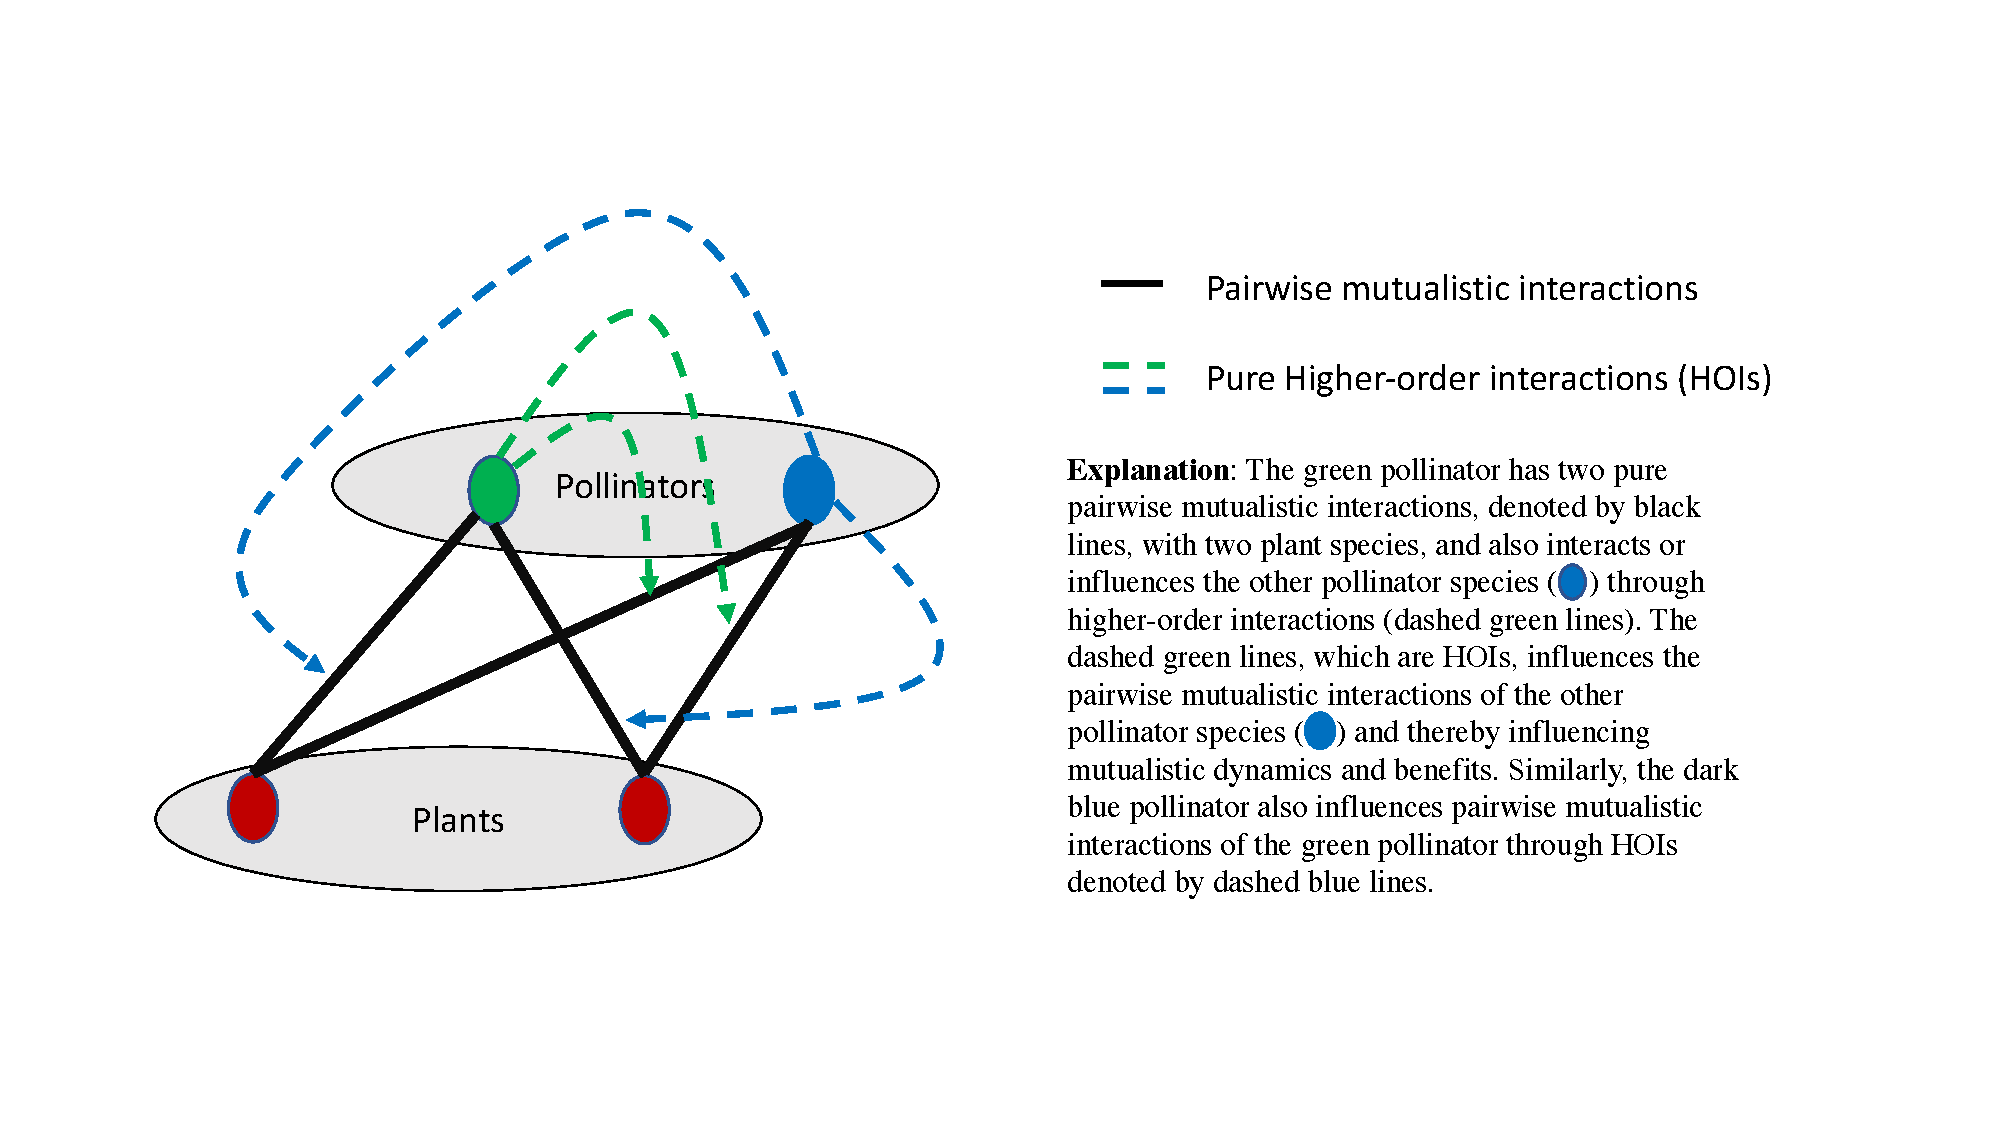
\includegraphics[width=15cm]{fig1.pdf}      
\end{center}
\caption{Representation of higher-order and pairwise mutualistic interaction in a simple mutualistic community of two pollinators and two plant species. Mutualistic interactions between species are mediated through mean phenotype modelled above}
\end{figure}


Higher-order interactions are intereactions that are not direct but influence pairwise interactions. Here in the figure 1 pairwise interactions are being influenced by a third species. Also we are considering only interactions that are mediated by one guild of species, here the pollinators. This is in a way saying that when a pollinator is interacting with a plant species, a third pollinator can thereby come and inhibit their interaction through disturbance, or through hovering around the plant species thereby limiting or minimising the plant-pollinator interactions. This is one example and there can be many ( have to think).We also assume that the higher-order interactions are only mediated by the pollinators and not by the plants, since pollinators are more mobile and thereby could influence plant-pollinator pairwise interactions? THis is one assumption and we can also relax this assumption.

Another assumption is that higher-order interactions are pure. This means that individuals belonging to the same pollinator species CANNOT influence pairwise pollinator-plant interactions of the same species. This assumption can also be relaxed easily. 

Next, we can further rewrite equation 6 as:


\begin{equation}
    \frac{dN_{i}}{dt} = N_{i}(t) \Bigg( \bar{b_{i}} -  \sum_{j}\alpha_{ij}N_{j} + \int\int\sum_{k} \frac{\gamma(z,z')}{1+ h\gamma(z,z')} p_{j}(z',t)p_{i}(z,t)dzdz' - \sum_{k}\sum_{l \neq k} \beta_{ikl}N_{k}N_{l}\Bigg) 
\end{equation}
where, $\beta_{ikl}N_{k}N_{l}$ is the term that captures the higher-order interactions. $\beta_{ikl}N_{k}N_{l}$ represents how species $l$ influences the pairwise interactions of species $i$ and species $k$. The two summations goes over species belonging only to the guild of pollinators and not the plants In our model formulation we assume that HOIs are only influenced by the pollinator species in a way that the interactions are trait-independent. This means that a pollinator species need not have a phenotype that is similar to the phenotype of the plant species to influence pairwise mutualistic interactions. THis means that one can simply model the HOIs  $\beta_{ikl}N_{k}N_{l}$ to be random numbers in a way that also takes a large sample of interactions into account. On the contrary, one can also model the HOIs to be trait-dependent. In this particular case, one can assume HOIs to be a three-way trait interaction between plants, a pollinator and a third pollinator of the form of multivariate gaussian interaction kernel $\beta_{ijk}(z,z',z'')$ where $z, z', z''$ are the phenotypes of a plant individual, a pollinator individual and a third pollinator individual. 
But for simplicity lets just consider for now that the HOIs are trait-independent. In that case, the evolutionary trait dynamics will thus be not influenced directly by such HOIs but only indirectly through changes in population dynamics. So for evolutionary dynmaics we can still use equation 7 for the dynamics of the mean trait:

\begin{equation}
    \frac{du_{i}}{dt} = h_i^2 \sigma_i^2\frac{\partial}{\partial u_{i}(t)}\bigg( \bar{b_{i}} + \int\int\sum_{k} \frac{\gamma(z,z')}{1+ h\gamma(z,z')} p_{j}(z',t)p_{i}(z,t)dzdz'\bigg)
\end{equation}


\section{Spatial context of mutualistic interactions}
In the presence of HOIs the metacommunity dynamics of mutualistic interactions can be written as:


\begin{equation}
    \frac{dN_{i}^k}{dt} = N_{i}^k(t) \Bigg( \bar{b_{i}^k} -  \sum_{j}\alpha_{ij}^kN_{j}^k + \int\int\sum_{k} \frac{\gamma^k(z,z')}{1+ h\gamma^k(z,z')} p_{j}^k(z',t)p_{i}^k(z,t)dzdz' - \sum_{l}\sum_{m \neq l} \beta_{ilm}^kN_{l}^kN_{m}^k\Bigg) + M_{i}^k - a N_{i}(t)^k
\end{equation}

where $M_{i}^k$ is the immigration of species $i$ from habitat patch $k$, $a$ is the dispersal rate of the species $i$ and $aN_i(t)^k$ is the term that captures emigration from natal patch $k$ (see Thompson et al 2017 Ecography, Thompson et al 2020, Eco. letters). Specifically following Thompson et al 2020. Eco. Letters, 

$$ M_{i}^k = a \sum_{j \neq k}^{n}\frac{e^{-rd_{jk}}}{\sum_{f\neq k}e^{-rd_{fk}}}N_i^j$$

Following this above formulation, more than one dispersal route can be taken during a particular time step. $d_{jk}$ was  is the distance between two patches j and k. Distance between patches decreases exponentially and the rate at which it decreases is captured by the parameter $r$. We could fix $r$ at $0.5$ in our model, which typically indicates global dispersal.


The evolutionary trait dynamics of mean trait $u_{i}(t)^k$ due to mutualistic interactions and dispersal can be written then as :


\begin{equation}
    \frac{du_{i}^k}{dt} = h_i^2 \sigma_i^2\frac{\partial}{\partial u_{i}^k(t)}\bigg( \bar{b_{i}^k} + \int\int\sum_{k} \frac{\gamma^k(z,z')}{1+ h\gamma^k(z,z')} p_{j}^k(z',t)p_{i}^k(z,t)dzdz'\bigg) -  h_i^2 \sigma_i^2 a \sum_{j \neq k}^{n}\frac{e^{-rd_{jk}}}{\sum_{f\neq k}e^{-rd_{fk}}} \frac{N_i^j}{N_i^k} u_{i}^j - \sum_{j}a\frac{N_i^j}{N_i^k} u_{i}^k
\end{equation}


\section{Possible questions}

1. How does co-evolutionary dynamics play out in the presence of individual variation and in the presence of HOIs? How does evolutionary trait patterning takes place in the presence of myriad interactions?

2. Do the presence of HOIs stabilize or destabilize co-evolutionary dynamics of mutualistic networks?


3. In the spatial context, how does local and regional processes shape ecosystem functions like biomass, species richness in the presence of individual variation, and in the presence of HOIs?

4. How does dispersal rate influence patterning of trait and turnover of species in the spatial meta mutualistic networks?

5. Any other possible questions??


\end{document}